% This example An LaTeX document showing how to use the l3proj class to
% write your report. Use pdflatex and bibtex to process the file, creating 
% a PDF file as output (there is no need to use dvips when using pdflatex).

% Modified 

\documentclass{l3proj}
\usepackage{cite}
\usepackage{graphicx}
\usepackage{float}
\graphicspath{ {./images/} }


\begin{document}

\title{Thales Sensor Mapping Demonstration Software}

    \author{Krasimir Ivanov\\
        Mohammad Atbaan Akhtar \\
        Shahzeb Zafar \\
        Shayam Nitin Bhudia \\
        Vrinda Sharma\\ 
        Krishang Patney\\}

\date{April 9, 2021}

\maketitle

\begin{abstract}

    This paper presents a case study of the development of a sensor mapping software, proposed by Thales UK. We discuss the proposal, the application made, the software development process and finally our insights and the conclusions drawn from the project as a whole.

\end{abstract}

%% Comment out this line if you do not wish to give consent for your
%% work to be distributed in electronic format.
\educationalconsent

\newpage

%==============================================================================
\section{Introduction}

This paper presents a case study of the development of a sensor mapping software. The application takes data from a sensor system like the SOPHIE LITE Electrical External ICD device \cite{sophie}. The application takes in the scan data and maps it onto a 3D or a 2D map to visualize the scanned data. Furthermore, the mapping function can simulate the sensor system.

The paper begins with some background information about our customer and their proposal (section 2 \& 3). It then delves into details about our main application followed by a thorough recount of the software development process (sections 4 \& 5). 

This is followed by our reflection about the project and key insights gained throughout the six to seven months of development (section 6). We finally conclude it with a brief look at the various software development practices we adopted and how closely our project’s progress was tied to the Professional Software Development course (section 7).


%==============================================================================
\section{Our Customer}

Thales Group is a French multinational company, founded in December 2000, that designs and builds electrical systems and provides services for the aerospace, defense, transportation, and security markets.\cite{thales} The proposal that was given to our team, CS01, by the company’s UK branch. Thales UK\cite{thalesUK} approached the University of Glasgow Computer Science department to task a student development team to build a proof of concept of sensor data visualization and simulation application.

Our customers consisted of Ian James, Iain Carrie, Matt Tucknott, and Christopher Dickson. Ian acted as our main point of contact and sponsor on behalf of Thales. Iain is the Project Technical Lead for Urban Canyon, one of Thales’ many ongoing projects, and was the main beneficiary of our application. Matt is a Thales Technical Expert on Geographic Information Systems (GIS)\cite{gis}  and has had over 20 years of experience in the field as well as 29 years of Java and C++. Christopher is a Thales Algorithms Engineer with over 19 years of software experience and has 10 years of experience with image processing.

The way our customer’s team was structured was that Ian would be our main liaison. Most of our conversations were with him and he was the first to be informed of any issues or scheduling details for meetings from our end. Iain was the one who approved of or suggested many of our application’s features earlier on during development while Christopher and Matt provided development support. Matt in particular was integral for fixing one of the major roadblocks we faced over halfway through development (more on this later). 

%==============================================================================
\section{The Project Proposal}

Thales UK was looking for software to support a sensor system with mapping information in 2D and 3D with potential real-time information update capability. Their long-term aim was to bring autonomous and manned platforms closer together with the integrated sensor and mapping software they proposed. The proposed project specification first aimed to develop a simple overlay of a target locator sensor on a map and then aimed to extend the integration to be 3D. The client stated that they were not constraining the development team on what technologies to use, however they would prefer that the mapping tool and the sensor suite be integrated to better aid their aim for the software to cope with a wide variety of situations.

The produced software solution is an open-source MIT licensed prototype, therefore a patent will not be sought. The main purpose and use of the software product are to provide proof of concept. The product will not be deployed into production, only used for demonstration purposes. The goal of the project proposal was to explore the technologies needed to develop such an application, what resources it needs, and to implement a prototype solution.

They stated that their goal for the first couple of iterations was to research available technologies for the framework of the application and what modules to use for the map and the mapping of the sensor information. This was aided by their recommendations on technologies as well as the availability of their software professionals, mapping, and sensing experts. After careful consideration and ranking of frameworks, the team initially settled on using the framework ElectronJS with Cesium, a 3D geospatial modeling tool, to start with.

%==============================================================================
\section{The Application}

Before we can discuss the application, we need to know the minimum viable product our customers expected. At the start of the first sprint, after our first meeting with the customer, we gathered the three major tasks, which would result in being the minimum viable product, with each of being split couple of sub-tasks. They were:

Task 1 - Establish a relationship between video and 2d (ground plane) map:
\begin{itemize}
	\item Task 1a: Populate a 2d radar plot (azimuth vs range) with detections obtained from a video. Assume 2d bounding box in the image, known calibration/pose of the camera, and known distance to object.  
	\item Task 1b: Annotate a 2d ground plane map with detections obtained from a video. As above, but plot on an open-source map based on known vehicle position/orientation. 
\end{itemize}

Task 2 - Establish a relationship between video and 3d map:
\begin{itemize}
	\item Task 2a: As Task 1b but remove the assumption of known distance to target and plot result on 3d map (or 2d ground projection of 3d map). Distance to target should be automatically determined by intersecting bearing from known bounding box with a ground plane as defined by the 3d map. Report the range to target.
	\item Task 2b: Project all visible rays from a camera onto 3d map and display total visibility from the current position. Assume knowledge of camera calibration, camera field of view, and camera/vehicle pose. 
\end{itemize}

Task 3 - Plot features from 3d map onto a video feed:
\begin{itemize}
	\item Task 3a: For an object positioned on the 3d map, determine and display its location in the video feed. Assume known calibration/pose of camera + known vehicle position. 
	\item Task 3b: Combining Tasks 2b and 3a determine whether the object identified in 3d map is visible to the camera and if not highlight that it is a hidden target.   
\end{itemize}

Along with this, we had also been asked to provide additional functionalities if time permits, they also requested to make the application open-source. To fulfill our tasks and carry out the request, we were recommended several APIs and software by our customers. Initially, we settled on CesiumJS and ElectronJS but over halfway through the project’s development lifecycle, we switched to our ArcGIS + JavaFX based application due to the limitations of our earlier approach, now called ThalesArc.

\subsection{ElectronJSApp}
This application had been made by combining a couple of technologies. The most notable being CesiumJS, which is an open-source JavaScript library for creating static or dynamic 2D and 3D maps,\cite{cesium} it supports for creating multiple maps which we deemed ideal for the intended use. Secondly, the front-end framework we used was Bootstrap, which allows for creating responsive websites, with a grid system, extensive prebuilt components, and powerful JavaScript plugins\cite{Bootstrap}. 

Both these technologies are combined and packaged under ElectronJS\cite{electron} an open-source software framework based on Chromium, which runs under the open-source JavaScript server runtime environment called Node.js\cite{Node.js}. 

This application is versatile, as Cesium can provide most of the data sets for 2D and 3D map features, we'd require. On top of this, the people at Cesium regularly update the extensive documentation with a sandbox feature to showcase their predominant features and how they can be integrated into a web-based application. A python script was first used to simulate sensor data and plot points on the map, but this was later scrapped in favour of an Android application we developed which could send actual geographical data gathered from a phone’s GPS to the application by utilising Web Sockets, this makes it possible to communicate between the application and user.

Cesium is a great API for displaying geospatial information within a web browser, making it lightweight, and easy to distribute on a massive scale, meaning it'd be great for displaying static data which does not change a lot, however, one of its major drawbacks is not being able to utilize the GPU on a computer, which would be the main platform for our application to be run on, this meant that having a constantly updating data stream would bog down the performance of the application, hence not being satisfactory enough for our vision of the product.

On top of the above-mentioned issues, we were also unable to project visibility rays within the 3D world hence not knowing where our targets would be located as they would be rendered in without having geospatial information attached to it. One of the solutions that'd allow us to overcome this roadblock would be to purchase the Cesium ion SDK licence\cite{ion}, therefore making it proprietary software and being over-budget.

These issues, combined with the application not deploying on anything but Windows, meant that we had reached the end of the road with Cesium and had to find a new approach to our project.

\subsection{ThalesArc}

ArcGIS Pro was our answer to Cesium’s shortcomings.\cite{arcgis} This is a geographic information system software developed by the Environmental Systems Research Institute (Esri)\cite{esri} which supports an API based on a 64-bit architecture and combines support for 2D and 3D applications, used for geospatial processing programs. Making it a great contender to the previously maintained ElectronJSApp application. ArcGIS Pro was integrated onto the JavaFX client application platform supporting cross-platform development and releases.\cite{javaFX}

The new application was everything we had hoped to achieve but failed to with the ElectronJSApp. This new API allowed us to project the field-of-view rays from the camera, whilst utilising the GPUs capabilities, hence allowing us to move the field-of-view cone around on the map just like a senor would be based on the geographic coordinate system.

Like before, a python script had now been modified to allow for sending JSON packets to the application which then converted them to Sensor objects, allowing us to have simulated data streams for plotting new user coordinates and target coordinates if given. However, due to time constraints, we were unable to further develop the Android simulator application to support the new ThalesArc app.

Whilst also completing the minimum viable product we were able to implement a few extra features which the customer had mentioned within their product requirements draft. This included adding a detailed log of all the targets being shown to the user, functionality of loading, creating, and saving these logs within the user's directory, and also additional features which can be further developed if wished by the customer, such as having target paths, which can be abstracted to also display the users routing.

\subsection{Application Comparisons}

Whilst writing down a few key features of the applications mentioned above would be a good enough explanation to a GIS expert, it can also easily confuse someone new to mapping technologies. Hence providing a more detailed explanation and comparison between the applications.

To realize our vision for the application it's beneficial to take a look at the wireframes developed within the first sprint of the software development lifecycle, which set out a concrete foundation for what the app would look like. As we can see in Figure 1, the wireframe is split into a few components, the left side is split off to log all the targets on the map, and a few more options for the user to choose between features and also displaying the current user location. The right side hosts the map which displays the field of view cone with the dead of ground information and users position.

\begin{figure}[!h]
    \caption{Sample wireframe}
    \centering
    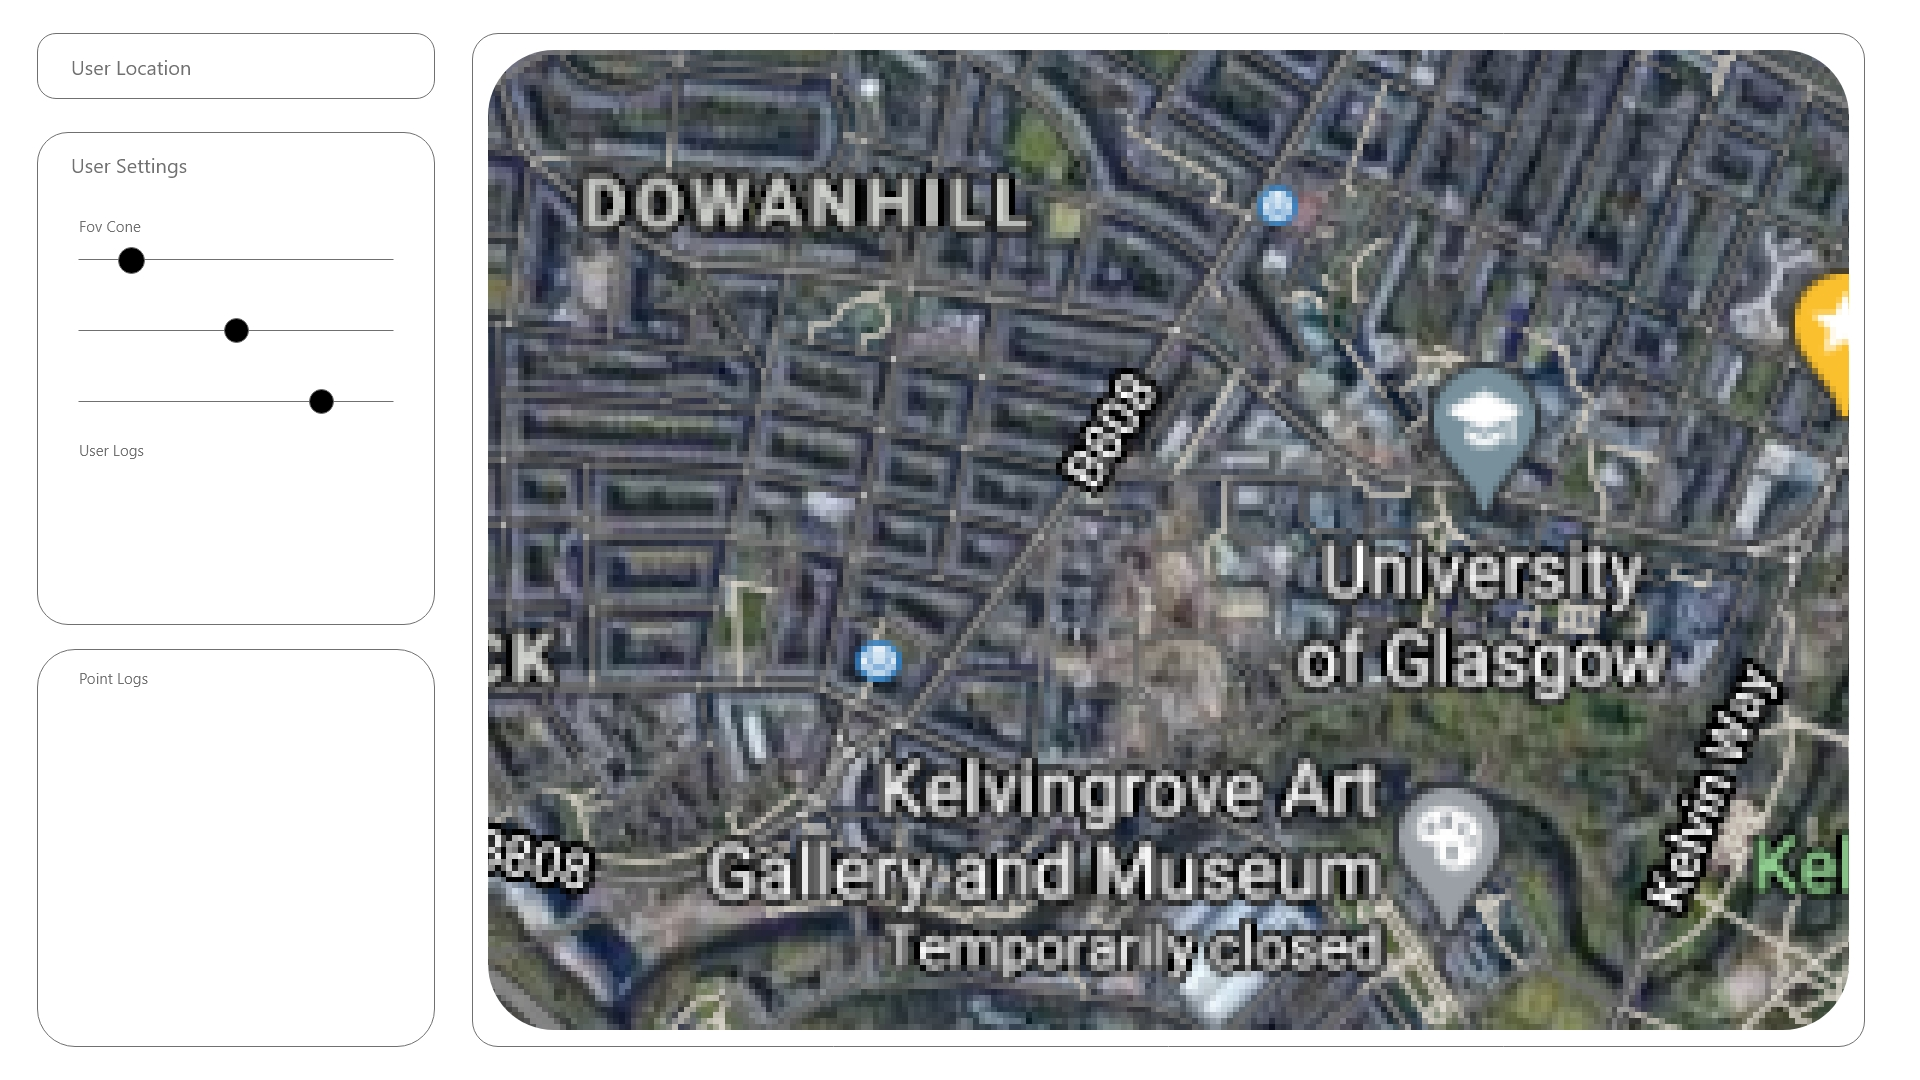
\includegraphics[width=0.7\textwidth]{wireframe.jpg}
\end{figure}

With the development of the product being split into two applications, starting with the first, ElectronJSApp. We've provided a 2D map starting in Glasgow. This application fulfils the customer's Task 1, which establishes a relationship between what a sensor can see which then gets plotted onto the 2D map, for example, we could spawn randomly generated points on to the map and a fixed user location. However, a big issue we faced is the points get generated onto a single graphic layer, combined with the map, resulting in computationally expensive graphic processing, which a web browser is not capable of. Especially if we wanted to have the constant stream of data coming in and updating the user's current location graphically while doing other processes. 

This segways into the second application we've developed as mentioned before which uses the ArcGIS Pro API. Which works in a more industry-standard fashion for mapping applications, where it uses data layers as a mechanism to display geographical datasets. The sample dataset we've used is located in Brest, France as it's provided by ArcGIS Pro out of the box.

\begin{figure}[!h]
    \caption{Example of layers in ArcGIS \cite{esri-layers}}
    \centering
    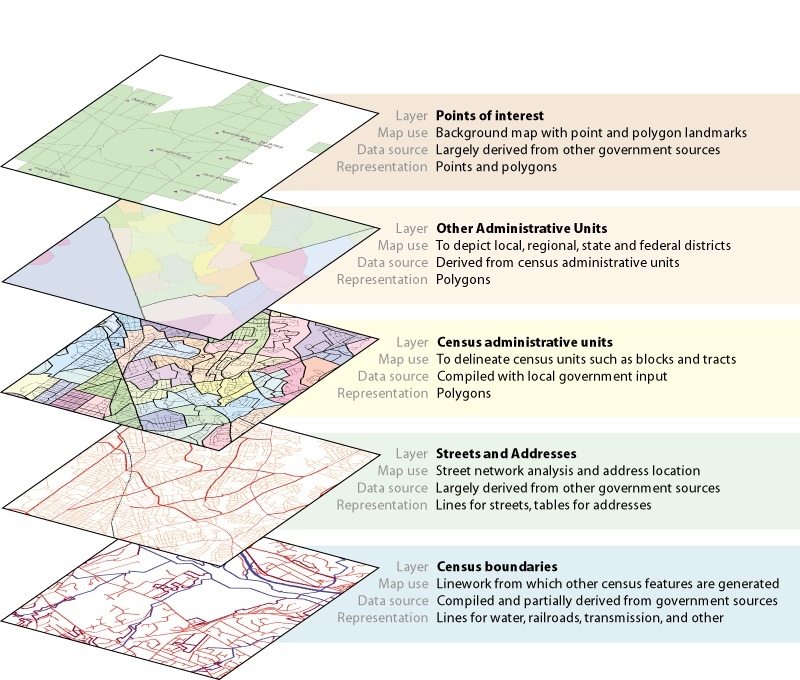
\includegraphics[width=0.3\textwidth ]{GISLayers.jpg}
\end{figure}

In figure 2 we can see different layers being are used in the image to display a few map features. Taking a note from this example we've personally used 3 main layers, one for each, the user, the targets and the field of view, with other additional layers for extra features. This allows us to dynamically or statically update each layer on its own hence reducing lag, and allowing us to use GPU resources to render the graphic layers in dynamically in real-time. 

\begin{figure}[H]
    \caption{ThalesArc line of sight visibility feature}
    \centering
    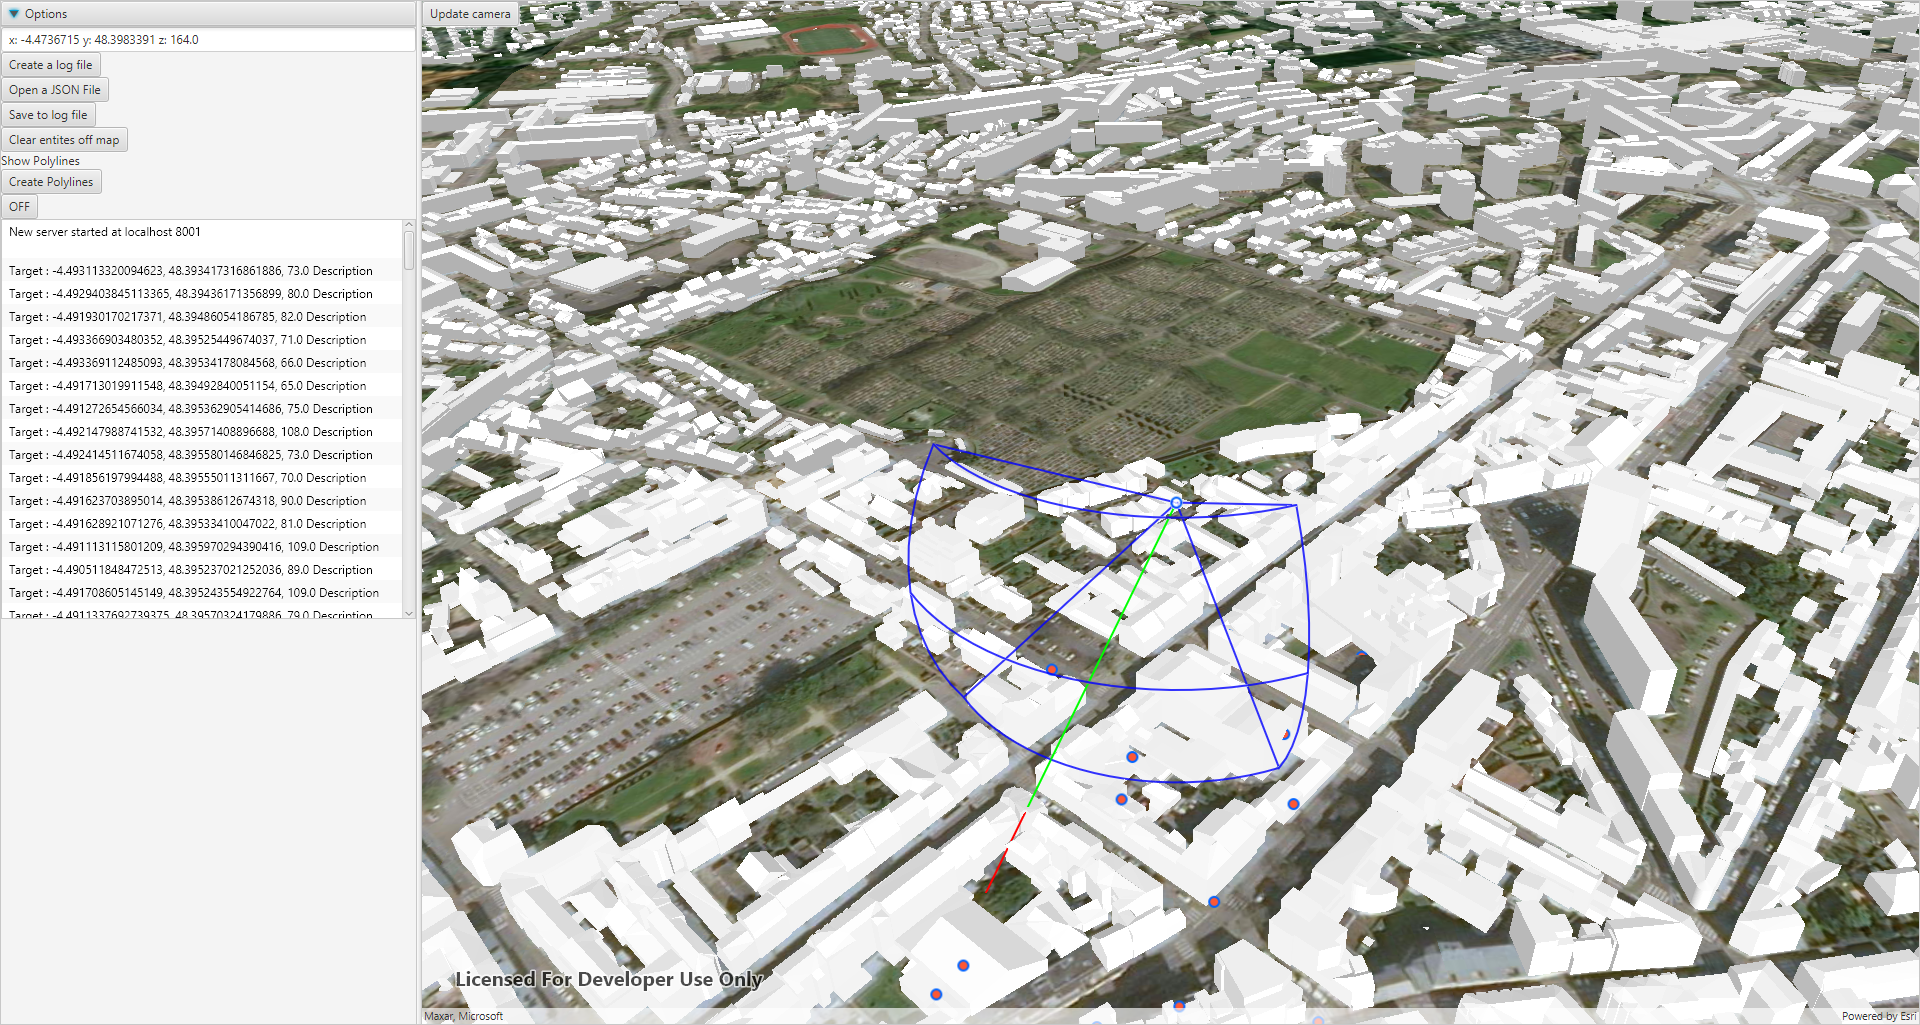
\includegraphics[width=\textwidth]{ArcGISLOS.jpg}
\end{figure}

Figure 3 showcases the feature, where we try and process the line of sight from a user to a target, which works by highlighting the line green if the point can be seen from the user and red if not.

\begin{figure}[H]
    \caption{ElectronJSApp line of sight visibility feature}
    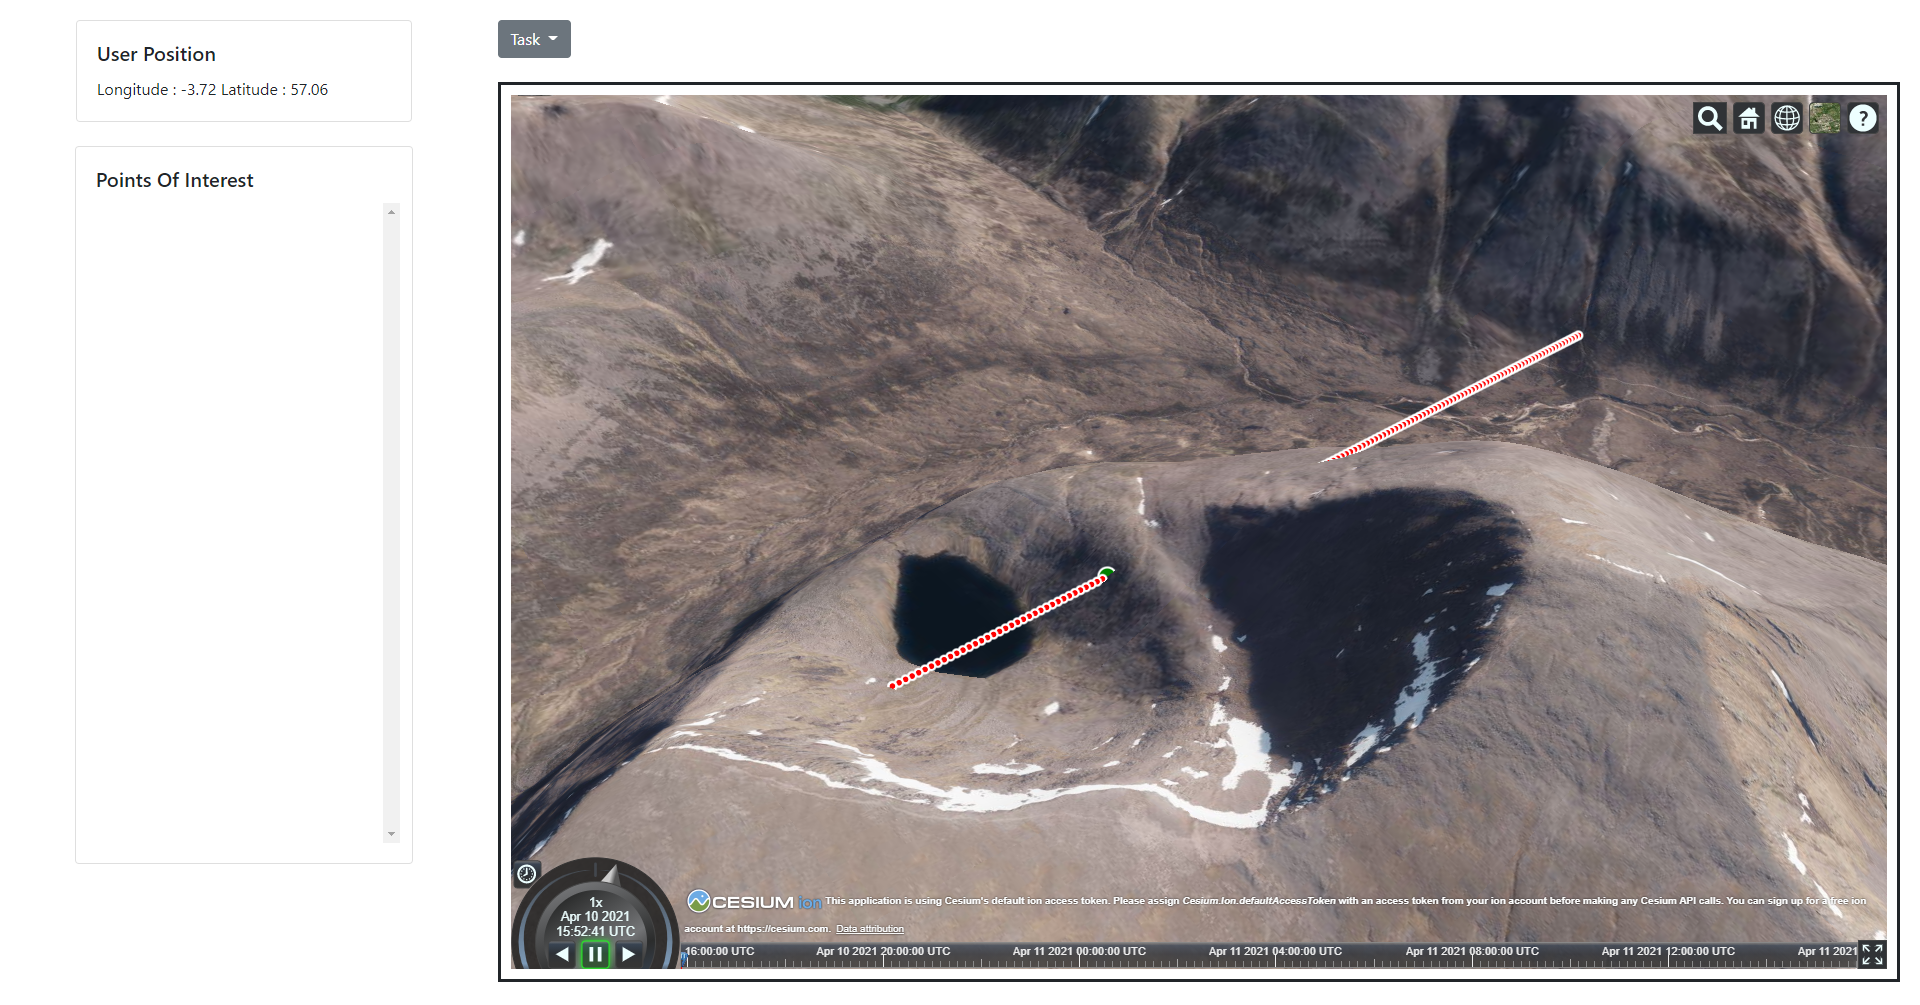
\includegraphics[width=\textwidth]{ElectronJSLOS.jpg}
\end{figure}

Trying to achieve this functionality in the ElectronJSApp required us to create many points in between the user and map to see whether or not it'd intersect with its surrounding terrain as seen in Figure 4. Whilst doing this process, the application gets resource hungry and start to bog down its overall performance. 

Other miscellaneous features that have been included are vector representation for targets, this can be abstracted to be used for the user's route or be disabled upon the users wish. Users can go back to the original user location by clicking the "Update Camera" button, they also have the freedom to create, save and update the log files which are stored in the "LogFiles" directory, for which a sample file has also been provided for demonstration.

%==============================================================================
\section{Software Development Process}

The development process the team used can be broken down into 4 sections. First, understanding the requirements given and formulating an action plan. Second, implementing the action plan, which was the development phase, that continued in parallel with the third phase which was testing the developed product. The fourth, and final phase, was the delivery of the produced software to the client.

\subsection{Understanding The Requirements And Forming A Plan}

As detailed in the Project Proposal section, a requirement was given to the development team by Thales UK, outlining a supporting software for a sensor system. The requirement stated that the purpose of the application was to be a demo which, if up to their standards, would then be used as a reference for a new product of their own for commercial purposes. In short, it is a proof of concept. The development team kept this in focus throughout the planning and execution of the project. Furthermore, it is worth noting that the team and the customer agreed that the produced software package will be open source. The licence to be used was left to our discretion so we settled for the MIT open-source licence\cite{mit}, as stated already in earlier sections, which was attached to the final product by the handover date. 
  
The implementation of the software product started with choosing a technology to work with, that was capable of supporting the proposed requirements and functionalities. Initially, this was the CesiumJS API and ElectronJS for creating the application (more details in Sections 4.1). Once the technology and the framework were chosen the development team proceeded to implement the requirements (i.e the tasks from Section 4) in a procedural order.

The basis for our team’s software development is the Agile\cite{agile} approach with Scrum\cite{scrum}. The entirety of the software development cycle was broken down into 5 sprints. A mandatory meeting with our customers was held before the start of each sprint. In each meeting, we discussed our progress, informed the customer of any current issues, and stated our goals and priorities for the following sprint. We also took any questions they had, answering them to the best of our ability, and showcased a live demonstration of the application(s) whenever we made a significant breakthrough.
 
At the end of a sprint, there was an evaluation of the work that had been done, a code review\cite{coder}, and a retrospective\cite{retro} to reflect on the sprint and the performance of the team members as well as determining if the goals of the sprint had been met. During the retrospective, the team listed the good, the bad, and the ok elements of the sprint and discussed ways of improving the departments in which we were lacking. The retrospectives were a crucial part of the team dynamic and in keeping the team on track to achieve the main goal of the project: the delivery of the software product while assuring quality.

Before any of this could happen, however, we needed to split the workload amongst ourselves. For this, we used assigned each member's roles either specified in Scrum or made arbitrarily by ourselves. Krishang and Krasimir assumed the roles of lead developers and UX designers. The two of them contributed a great deal to both the front and back end of the software, with Krishang going the extra mile by implementing unit tests and getting our CI/CD pipelines working. Vrinda was also a developer and made a companion Android application by herself while also acting as a quality assurance manager. Shayam took up the role of toolsmith and worked on this dissertation with Shahzeb who also acted as the product owner. Atbaan recorded all the meetings we had with the customer, took notes, and maintained our wiki. While the members of the team had equal standing, for the most part, Krishang also took on the responsibility of Scrum Master\cite{ScrumMaster} to keep everything well organised.

\subsection{The Development Phase}

Progress in the first couple of sprints was smooth. We got a handle on CesiumJS and were very successful in completing around half of the tasks assigned to us. There was constant communication between the team members and while initially, our pace was rather slow – understandably since all of us were quite new to a collaborative assignment such as this, and the lack of an actual, physical gathering due to COVID-19 didn’t help – we eventually got a hang of things and kept up with our schedule. The representatives from Thales UK liked what we were doing and for the sake of quality and efficiency, we also kept a steady line of communication with our sister team, CS22, to exchange ideas and troubleshoot any issues either of the teams may have.

However, our progress came to a screeching halt when the development reached task 2b. Due to Cesium’s limitations (see Section 4.1) we could not move any further and ended up wasting almost two whole sprints in trying to rectify our issues. Instead of working on the main application, most of the team was relegated to looking up possible solutions. Vrinda continued working on the Android application so that we had something to show to our customers.

Many avenues and resources were searched for scoured through in our quest to find a viable solution. The documentation for Cesium was extensively gone over and websites like Stack Overflow were frequently visited in hope of finding similar issues and their fixes. We also consulted team CS22 but their way of approaching our customer’s requirements was different from our own so they couldn’t help us much, but their efforts are still appreciated.

When our labour bore no fruit, we went to our customers for help. After an exchange of emails between the product owner and Ian James from Thales UK, a direct line of communication was established between the developers and Matt Tucknott (more details in Section 2 for both) who greatly assisted them in troubleshooting and eventually coming up with a solution to our conundrum.

The only way to fix our problem was to scrap our existing application and create a new one with the ArcGIS API (see Section 4.2). Time was of the essence. The team now knew what to do but had very little time to do it due to the sheer amount of time wasted prior. Working overtime, our developers quickly made headway towards the development of the new application. They flawlessly redid all of the work from before and near the end of the final sprint, they got most of the work done and even implemented some additional features not specified in the minimum requirement. What’s more, they kept a calm head and didn’t let the frustration they were no doubt feeling bleed into inter-team communications, thereby preserving the positive atmosphere and dynamic our team had.

\subsection{Quality Assurance And Project Management}
 
While successfully creating a working application is good and all, we also had to take care of the quality. The method that was used to ensure the consistent quality of the software and to root out bugs was testing. We tested our application in two ways: the traditional manual way, user testing; and an automated, robust method known as Unit testing \cite{unit}. The implemented tests had decent software coverage, though Unit testing was not used for UI testing \cite{uitest}, which was instead done manually by the team's testers.

Gitlab runners \cite{runner} were used to implement Unit testing for both the core applications and the CI/CD pipelines \cite{pipe}. The tests were run as jobs on a UNIX machine. The development team planned on having Unit test jobs running across the entire application. However, due to unforeseen hurdles during the development, test runners could not be set up for the display drivers. This meant the team could not set up pipelines successfully for the ElectronJSApp but we were successful in creating the ThalesArc application pipeline.

It needs to be noted that everything achieved this far – the planning, the development, and the testing for quality – could not have been done without some system of management \cite{management}. As mentioned earlier, there was not a single time when the team were physically gathered together. Not only that, not all of us were in the UK. We had to work around multiple timezones with many of our members facing internet issues. We made good use of MS Teams to communicate and arranged plenty of inter-team meetings to discuss the project and even have casual talks to keep up morale.

If a team member was busy or sick, they made sure to promptly let the rest of the team know so that someone could take over for them. Tasks were discussed among the team and everyone was free, even encouraged rather, to work on what they were comfortable with. Testers were rotated on a regular basis to catch more bugs. Communication with the customers was also kept up. There was a regular exchange of emails and a couple of meetings were also scheduled for a more thorough, non-time constraint discussion unlike during the customer meetings.

\subsection{The Final Presentation And Project Handover}
 
The project was concluded with a final presentation. Normally, during our customer meetings, the developers and the product owner were the ones who spoke. Here though, every member of the team got a chance to speak before a live audience. Shahzeb opened up with an introduction to the team and the customers; Vrinda discussed the motivation for the project, followed up by an explanation of the minimum viable product. Krishang explained the underlying technologies used and both he and Krasimir demoed the final product. We concluded with a few closing remarks read out by Shahzeb which was followed up by a QnA session with the marker, the customers, and the audience.

The presentation went great. Our customers from Thales UK were happy with the final product and greatly impressed by our effort to make a comeback from what seemed to be a colossal pitfall – a sentiment which our peers watching shared as well. Alongside this was a formal handover of the application to the customers via a release branch on Gitlab. Instructions on how to access said branch, download the software package, and set up the applications (ElectronJSApp and ThalesArc) were shared with them and the software was fully handed over, with the team not taking responsibility for further development and maintenance.

%==============================================================================
\section{Reflection and Insights}

Although there were many ups and downs throughout this project and many days of frustration, it was very insightful and a great learning experience. Here are some of the things the members of our team have to say regarding everything:

Krasimir: The project showed me the value of working in a team for a longer period of time. Furthermore, I learned how to go from a general project description to a complete application. I also improved my ability to gather requirements from customers which is vital in the industry.

Atbaan: This project has helped me understand how there is so much more to being a software developer than just programming. It taught me how to interact with customers and my teammates over a long time period and it gave me "real-world experience" while still studying at the university.

Shahzeb: My experience with the team project has been quite good. I met and got along with new people who I very much enjoyed working with. I got to experience some of the hardships that take place during the development of any software and gained a new appreciation for software developers. Most importantly, I learned a new set of skills that will come in handy should I ever take up software development in the future.

Shayam: The PSD group project shed light on what it takes to go through the software development process and product delivery. During the project, I learned about team dynamics, software management, among other things. Most importantly, I have gained good foundations to build on in future projects and teams.

Vrinda: This project really helped me understand the intricacies of the software development process which is crucial for working in the industry. Working with a team for over 6 months helped me understand the importance of teamwork and dividing the work efficiently to achieve more in less amount of time.

Krishang: The project helped me take a look into what software engineering practices could look like for a product that aims to be served as a demonstration tool, whilst also giving an insight into what it takes to create a product from the ground up while only being given a description of its potential features.



%------------------------------------------------------------------------------
\section{Conclusions}

The duration of the team project was quite long, with it spanning two whole semesters. During this time many of us were not in our comfort zone by working remotely and team dynamics took a while to establish. But as our team has stated in Section 6, we learned a lot from our time working together and feel that it’s been a great experience all things considered.

The project was tied closely to the Professional Software Development course \cite{psd}. Many of the practices we adopted were first introduced during the course. We were unfamiliar with the new information and terminology at first and took a while to wrap our heads around it during the initial sprints but it wasn’t long before we grasped everything and started working in earnest as it is done in the industry.

Agile software development with Scrum was our bread and butter. Our workload was divided into short sprints and amongst the team members. We had continuous testing and we adapted to various upsets and modified our approach – thereby not stubbornly sticking to an ill-conceived plan. We held retrospectives to see where we stood and get everyone on the same page and made good use of branching to manage our Gitlab repository.

In that regard, I can confidently state that we meticulously followed the guidelines provided by the PSD course, while also making adaptations of our own to efficiently produce the software required by our customers and deliver it, especially since this was our first time doing anything of this scale with an actual, real-world customer.

The mistakes we made and tribulations we went through gave us a deeper understanding of the professional side of Computer Science and taught us not to underestimate our chosen career path. The experience gained here is essential for our growth and will most likely provide us with a solid foundation to stand on should any of us ever dip our toes into the vast world of software development.

We are thankful for the guidance provided by our coach Raghad Abdul Rab; our markers Paul Siebert and Jesus Rodriguez Perez; and our PSD lecturer Tim Storer. We also appreciate our customers from Thales UK for being great sports by treating us as equals and not looking down on us for being “students”.

\newpage

%==============================================================================
\bibliographystyle{plain}
\bibliography{dissertation}
\end{document}
